\section{Debugger/GUI}
\label{sec:debugger}

\vonda comes with a GUI \citep{rudibuggerThesis} that helps navigating, compiling and editing the source
files belonging to a project. It uses the project file to collect all the
necessary information.

\begin{figure}[thb]

  \centering
  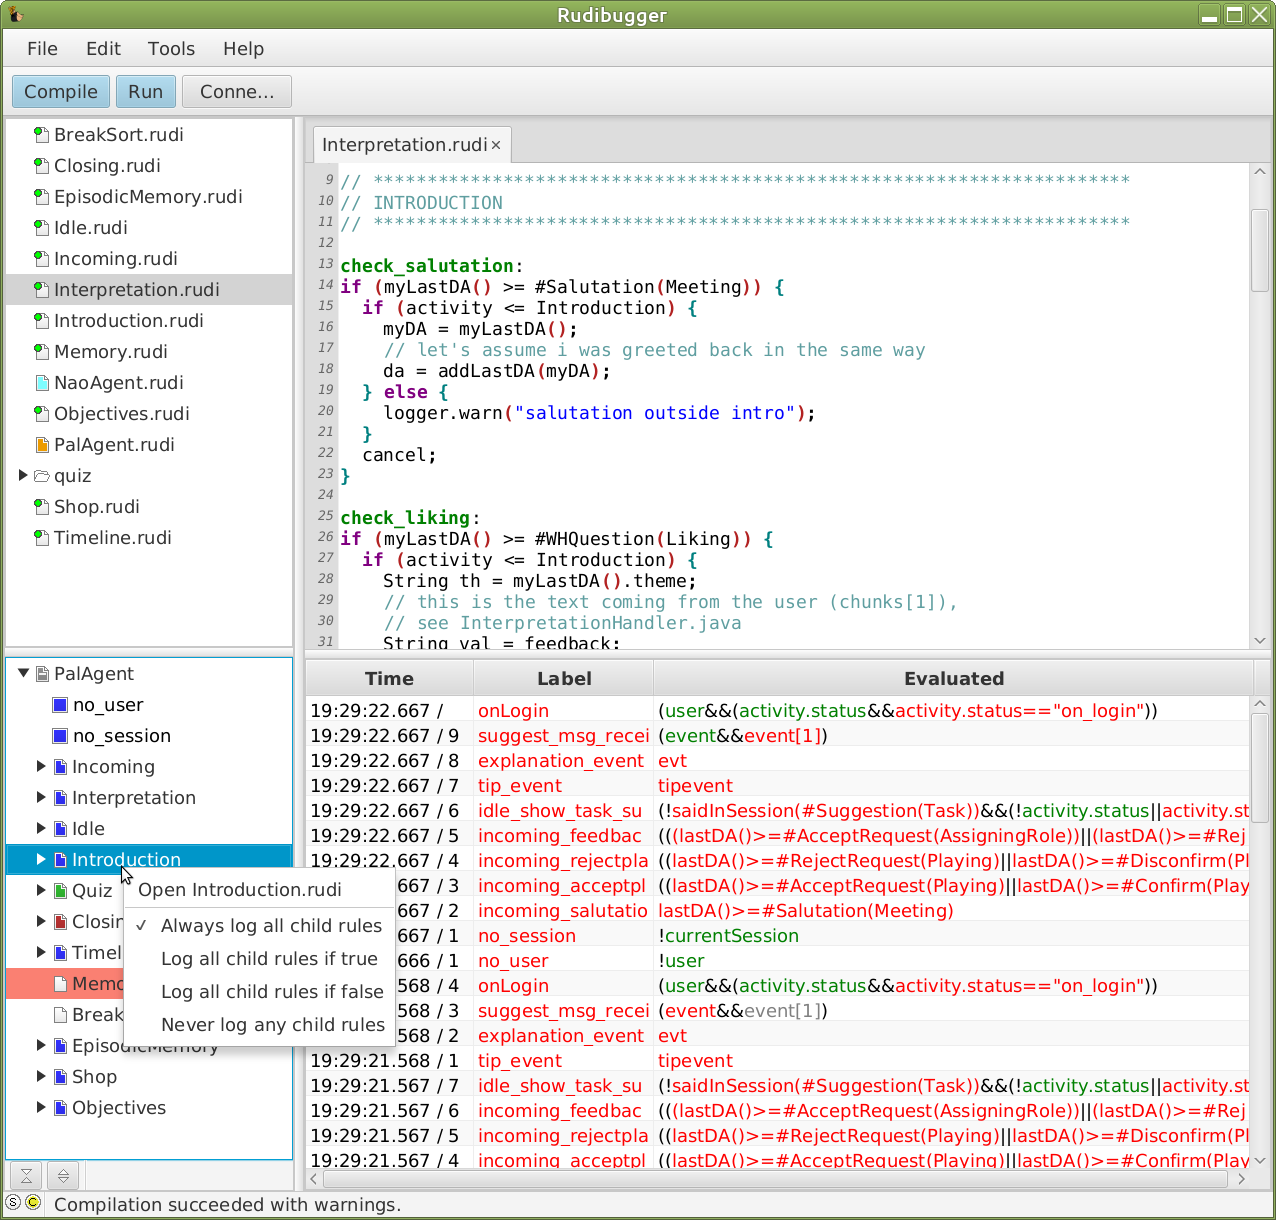
\includegraphics[width=.8\textwidth]{VondaGui.png}
  \caption{The \vonda GUI window}
  \label{vondagui}
\end{figure}

% Writing / Compilation part

Upon opening a project, the GUI displays the project directory (in a
\textit{file view}).  The user can edit rule files from within the GUI or with
an external editor like Emacs, Vim, etc.  and can start the compilation
process. After successful compilation, the project view shows what files are
currently used, and marks the top-level and the wrapper class files. A second
tree view (\emph{rule view}) shows the rule structure in addition to the module
structure. Modules where errors or warnings were reported during compilation
are highlighted, and the user can quickly navigate to them using context menus.

% Live system part

Additionally, the GUI can be used to track what is happening in a running
system. The connection is established using a socket to allow remote debugging.
In the rule view, multi-state check boxes are used to define which rules should
be observed under which conditions. A rule can be set to be logged under any
circumstances, not at all or if its condition evaluated to true or to
false. Since the rules are represented in a tree-like structure, the logging
condition can also be set for an entire subgroup of rules, or for a whole
module. The current rule loggging configuration can be saved for later use.

The \emph{logging view} displays incoming logging information as a sortable
table. A table entry contains a time stamp, the rule's label and its
condition. The rule's label is colored according to the final result of the
whole boolean expression, and each base term is colored accordingly, or greyed
out if short-cut logic led to premature failure or success of the expression.
